\section{What we have done}

\begin{frame}{Modelling}

    \only<1,2>{
        We derived the \textbf{equations of motion} of the Magnetic Levitation System (MLS) based on a Lagrangian approach.
    }

    \only<1>{


        \begin{equation}
            \frac{d}{dt} \left( \frac{\partial \mathcal{T}}{\partial \dot{\mathbf{u}}} \right) - \frac{\partial \mathcal{T}}{\partial \mathbf{u}} + \frac{\partial \mathcal{D}}{\partial \dot{\mathbf{u}}} + \frac{\partial \mathcal{U}}{\partial \mathbf{u}} = \mathcal{Q}
            \label{eq:lagrange_equation}
        \end{equation}

        \begin{equation}
            \begin{aligned}
                \mathcal{T} & = \frac{1}{2} m \dot{z}^2 + \frac{1}{2} L_1(z, \dot{q_1}) \dot{q_1}^2 + \frac{1}{2} L_2(z, \dot{q_2}) \dot{q_2}^2                                                                             \\
                \mathcal{D} & = \int_{\dot{z}(\cdot)} \frac{1}{2} C_d A \rho \dot{z}^2 d\dot{z} + \int_{\dot{q_1}(\cdot)} R_1(\dot{q_1}) \dot{q_1} d\dot{q_1} + \int_{\dot{q_2}(\cdot)} R_2(\dot{q_2}) \dot{q_2} d\dot{q_2} \\
                \mathcal{U} & = -m g z - q_1 V_1 - q_2 V_2                                                                                                                                                                  \\
                \mathcal{Q} & = 0
            \end{aligned}
        \end{equation}

    }

    \only<2>{
        \begin{equation}
            \begin{cases}
                m \ddot{z} - \frac{1}{2} \frac{\partial L_1}{\partial z} \dot{q_1}^2 - \frac{1}{2} \frac{\partial L_2}{\partial z} \dot{q_2}^2 + \frac{1}{2} C_d A \rho \dot{z} |\dot{z}| - m g = 0                                                                                                                                                                                                            \\
                \frac{1}{2} \left( \frac{\partial^2 L_1}{\partial \dot{q_1} \partial z} \dot{z} + \frac{\partial^2 L_1}{\partial \dot{q_1}^2} \ddot{q_1} \right) \dot{q_1}^2 + \frac{\partial L_1}{\partial \dot{q_1}} \dot{q_1} \ddot{q_1} + \left( \frac{\partial L_1}{\partial z} \dot{z} + \frac{\partial L_1}{\partial \dot{q_1}} \ddot{q_1} \right) \dot{q_1} + L_1 \ddot{q_1} + R_1 \dot{q_1} - V_1 = 0 \\
                \frac{1}{2} \left( \frac{\partial^2 L_2}{\partial \dot{q_2} \partial z} \dot{z} + \frac{\partial^2 L_2}{\partial \dot{q_2}^2} \ddot{q_2} \right) \dot{q_2}^2 + \frac{\partial L_2}{\partial \dot{q_2}} \dot{q_2} \ddot{q_2} + \left( \frac{\partial L_2}{\partial z} \dot{z} + \frac{\partial L_2}{\partial \dot{q_2}} \ddot{q_2} \right) \dot{q_2} + L_2 \ddot{q_2} + R_2 \dot{q_2} - V_2 = 0 \\
            \end{cases}
        \end{equation}
    }

    \only<3>{
        In order to simplify the model, we have \textbf{neglected the effect of the current on the value of the inductances (strong assumption)}.
        We also have neglected any velocity linearly dependent terms in the equations of motion.

        \begin{equation}
            \begin{cases}
                \frac{\partial L}{\partial I}     & \approx 0 \\
                \frac{\partial^2 L}{\partial I^2} & \approx 0 \\
                \dot{z}                           & \approx 0
            \end{cases}
            \label{eq:model_reduction_conditions}
        \end{equation}

        \vspace{9pt}

        From literature, we also have found an experimental based model for the inductances.

        \begin{equation}
            L = L(z) = L_0 + L_z e^{-a_z z}
        \end{equation}

    }

    \only<4>{
        The current model is a simplified version of the original one, but from experimental data we can see that it's still \textbf{able to capture the main dynamics of the system}.

        \begin{equation}
            \begin{cases}
                \dot{z} = v                                                                                                                                 \\
                \dot{v} = m^{-1} \left(\frac{1}{2} \frac{\partial L_1}{\partial z} I_1^2 + \frac{1}{2} \frac{\partial L_2}{\partial z} I_2^2 + m g  \right) \\
                \dot{I_1} = L_1^{-1} \left(- R_1 I_1 + (k_1 U_1 + c_1) \right)                                                                              \\
                \dot{I_2} = L_2^{-1} \left(- R_2 I_2 + (k_2 U_2 + c_2) \right)
            \end{cases}
            \label{eq:reduced_quations_of_motion_final}
        \end{equation}

        Notice that $z$ is the position of the ball (what we want to control), while $U_1$ and $U_2$ are the inputs of the system (what we can control).

    }

    \only<5>{
        The model has also been linearized and transformed in state-space form.

        \begin{equation}
            \begin{aligned}
                \dot{\mathbf{x}} & = f(\mathbf{x}, \mathbf{u}) \\
                \mathbf{y}       & = g(\mathbf{x}, \mathbf{u})
            \end{aligned}
            \quad
            \rightarrow
            \quad
            \begin{aligned}
                \dot{\delta\mathbf{x}} & \approx A \delta\mathbf{x} + B \delta\mathbf{u} \\
                \delta\mathbf{y}       & \approx C \delta\mathbf{x} + D \delta\mathbf{u}
            \end{aligned}
        \end{equation}

    }

\end{frame}



\begin{frame}{Parameters identification}

    \only<1>{
        In order to control the system, we had to \textbf{identify the parameters of the system}.
        To do so, many experiments have been conducted.
    }

    \only<2>{
        Control to Voltage mapping.

        \begin{columns}[c, onlytextwidth]

            \begin{column}{0.45\textwidth}

                As predictable, the control to voltage mapping is a linear function outside the `no control zone'.

                \begin{equation}
                    V = \begin{cases}
                        V_{min} & \text{if } U < U_{min}    \\
                        k U + c & \text{if } U \geq U_{min}
                    \end{cases}
                \end{equation}

            \end{column}

            \begin{column}{0.55\textwidth}

                \begin{figure}
                    \centering
                    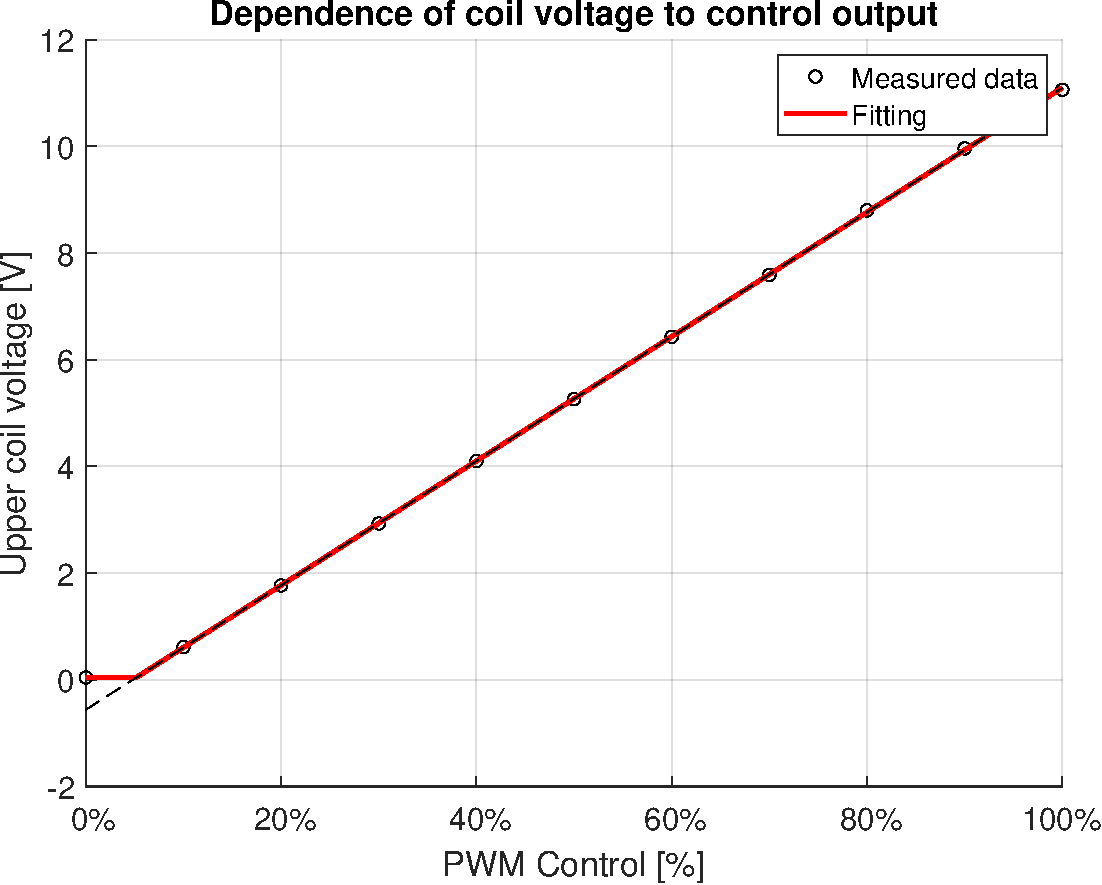
\includegraphics[width=0.8\textwidth]{img/MATLAB/measurements/control_to_voltage.pdf}
                    \caption{Voltage as a function of $U$}
                \end{figure}

            \end{column}

        \end{columns}

    }

    \only<3>{
        Electromagnetic force characterizations.

        \begin{columns}[c, onlytextwidth]

            \begin{column}{0.65\textwidth}

                \begin{figure}
                    \centering
                    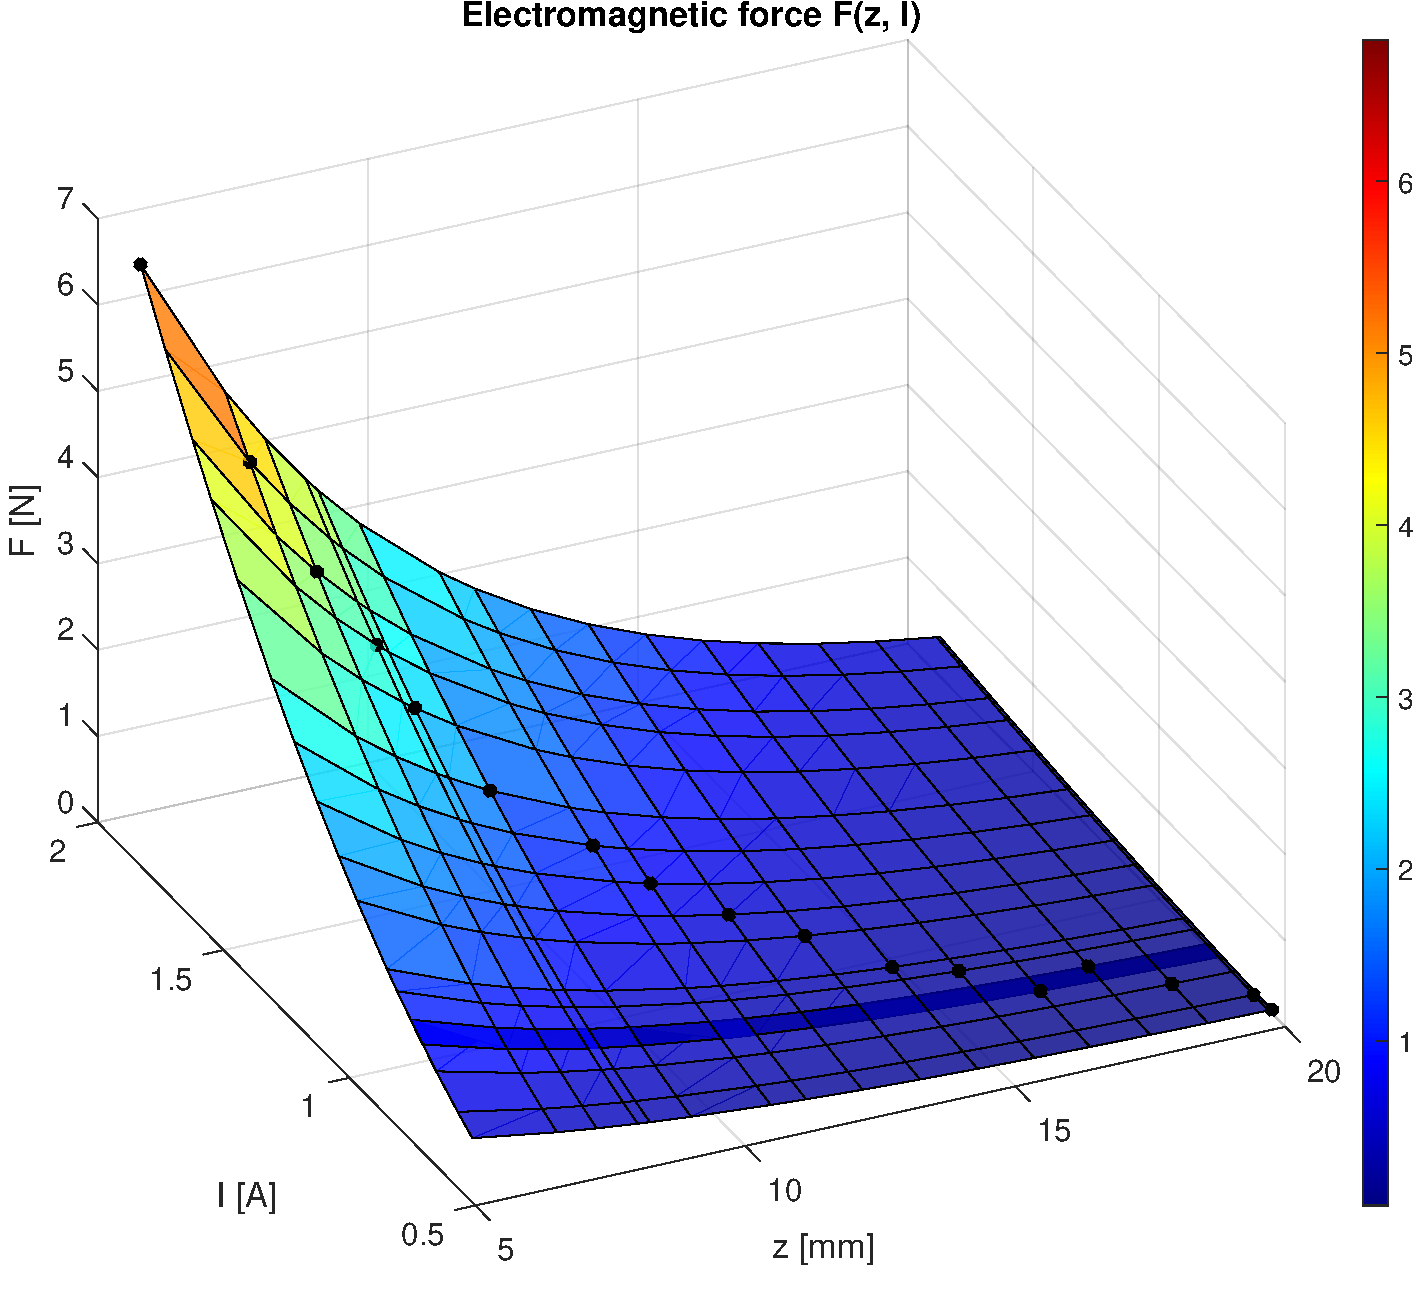
\includegraphics[width=0.8\textwidth]{img/MATLAB/measurements/force.pdf}
                    \caption{Electromagnetic force as a function of $z$ and $I$}
                \end{figure}

            \end{column}

            \begin{column}{0.35\textwidth}

                Notice that from the theoretical model, we have found the electromagnetic force acting on the ball to be:

                \begin{equation}
                    F_{em} = \frac{1}{2} \frac{\partial L}{\partial z} I^2
                \end{equation}

            \end{column}

        \end{columns}

    }

\end{frame}



\begin{frame}{Controlling}

    \only<1>{
        We have implemented a Simulink model of the system.

        \begin{figure}
            \centering
            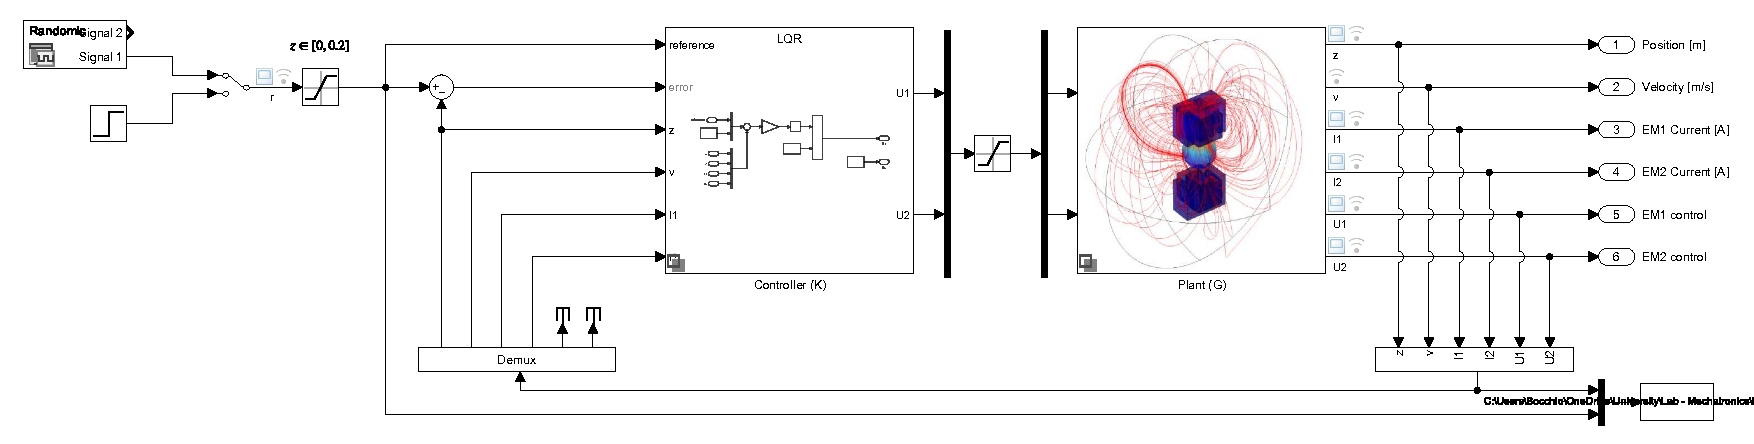
\includegraphics[width=1\textwidth]{img/MATLAB/simulink_model.pdf}
            \caption{Simulink root model of the Magnetic Levitation System}
        \end{figure}

        Some controllers have also been implemented and tested.

    }

    \only<2>{
        PID (both with and without anti-windup) controllers have been tested.

        \begin{figure}
            \centering
            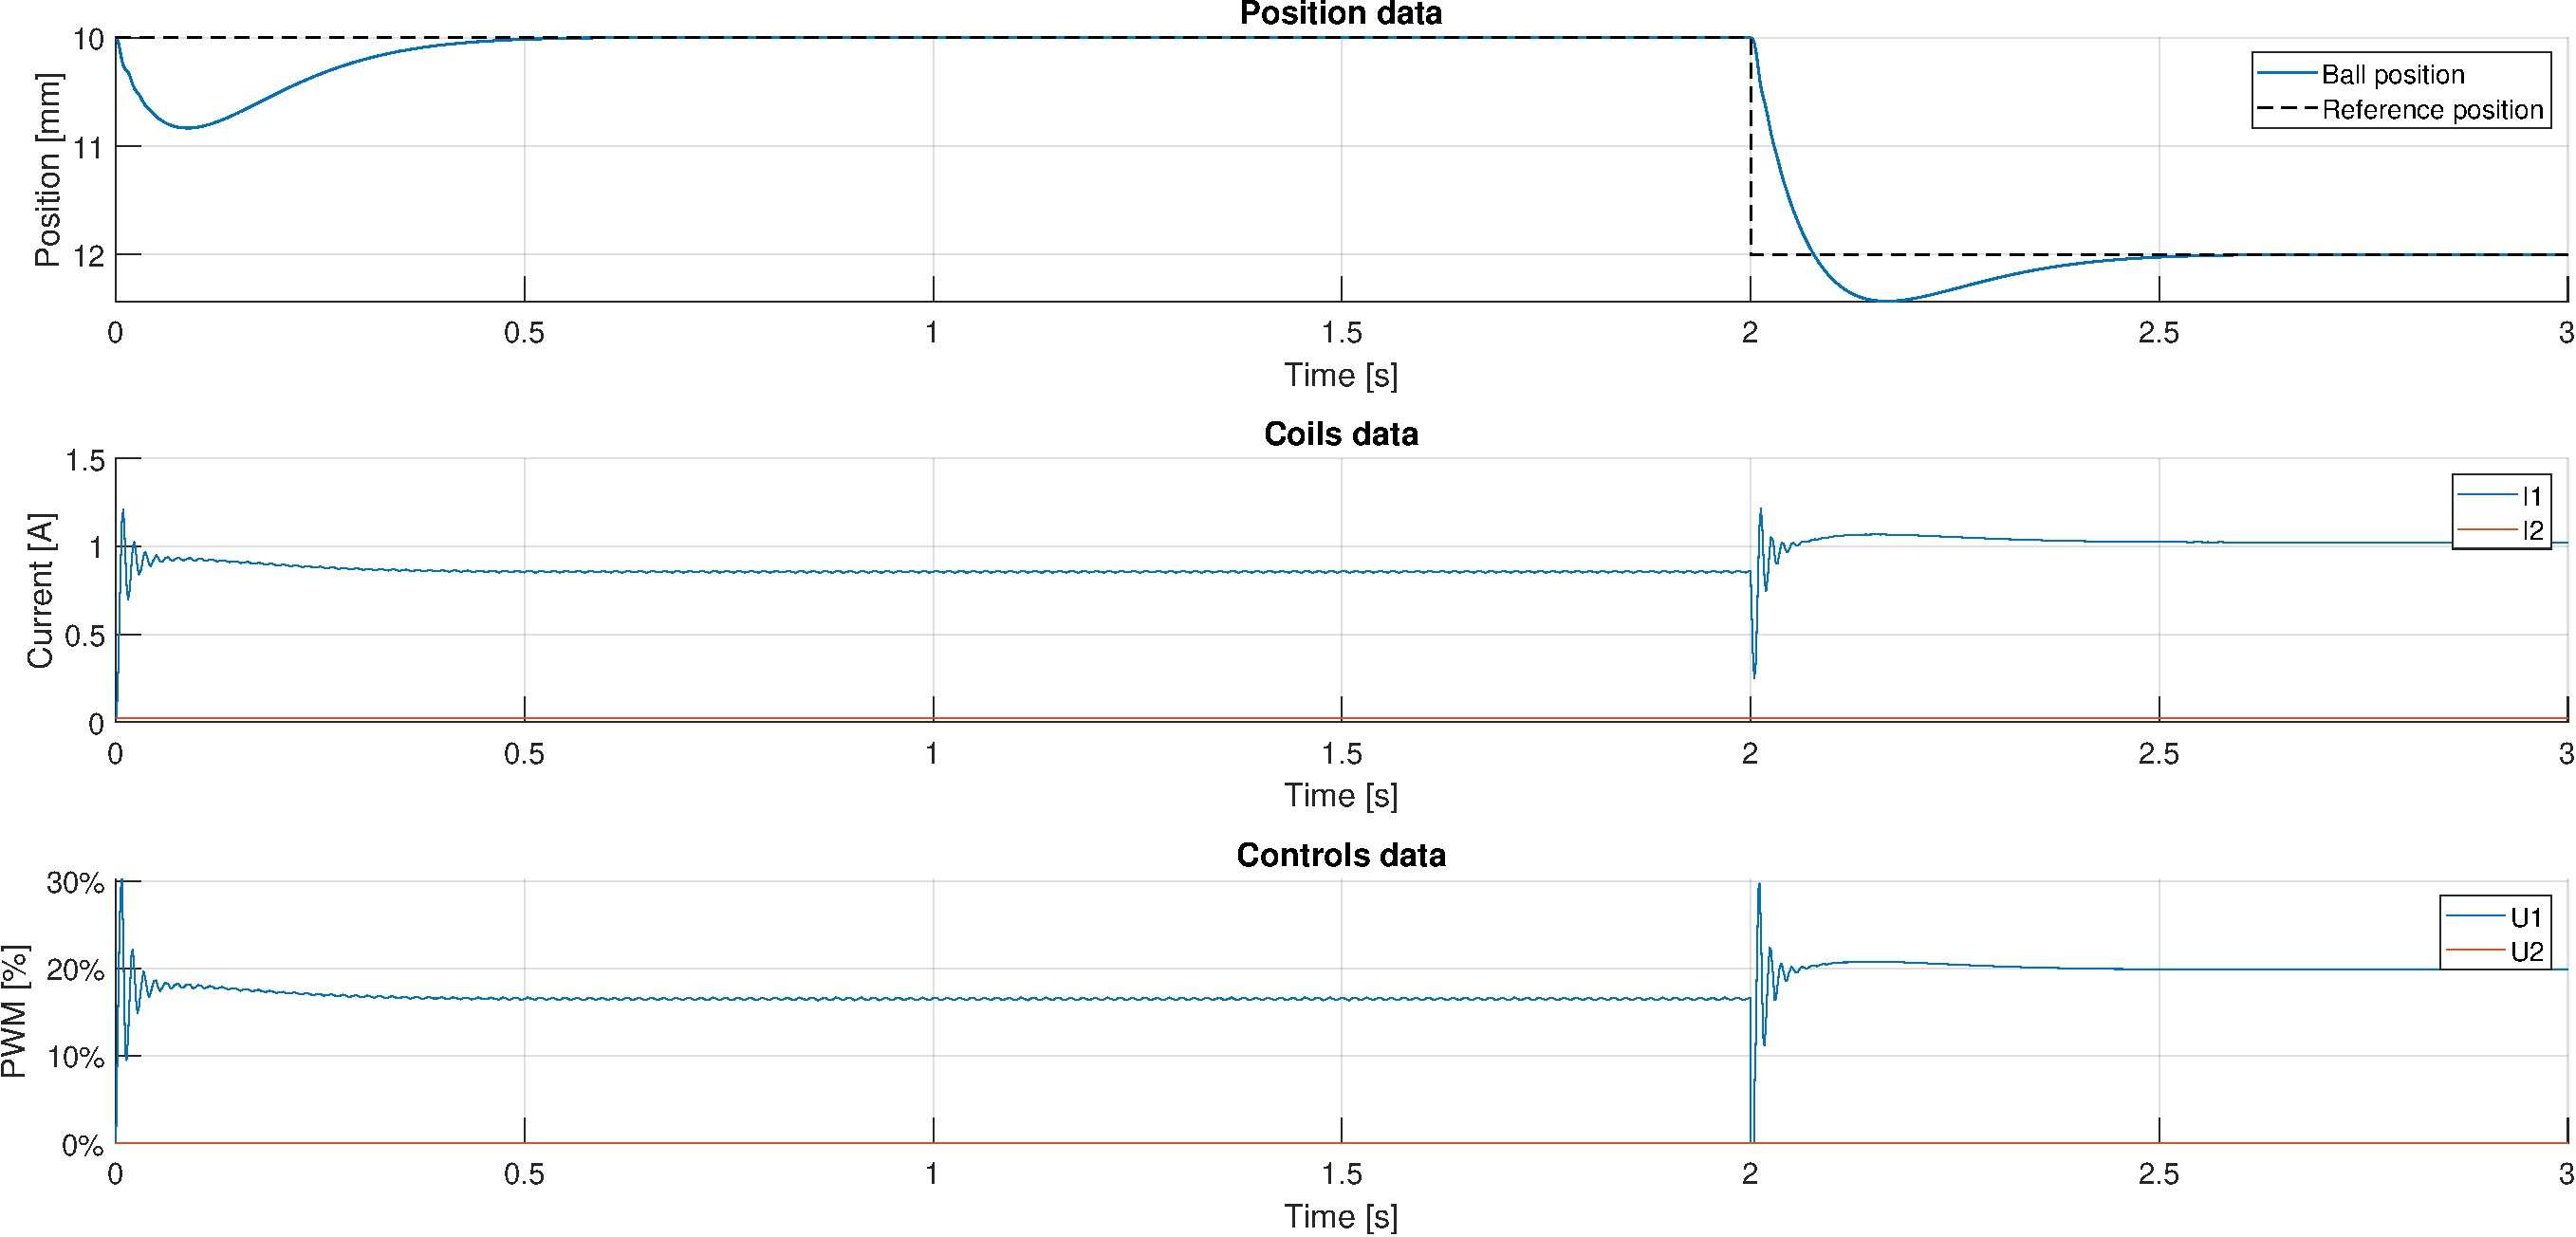
\includegraphics[width=1\textwidth]{img/MATLAB/runs/PID_anti_windup.pdf}
            \caption{PID with anti-windup controller}
        \end{figure}

        A PID controller without anti-windup has also been tested but with a clearly worse performance (strong oscillations around the reference).

    }

    \only<3>{
        LQR controllers with (limited) tracking capabilities have been tested.

        \begin{figure}
            \centering
            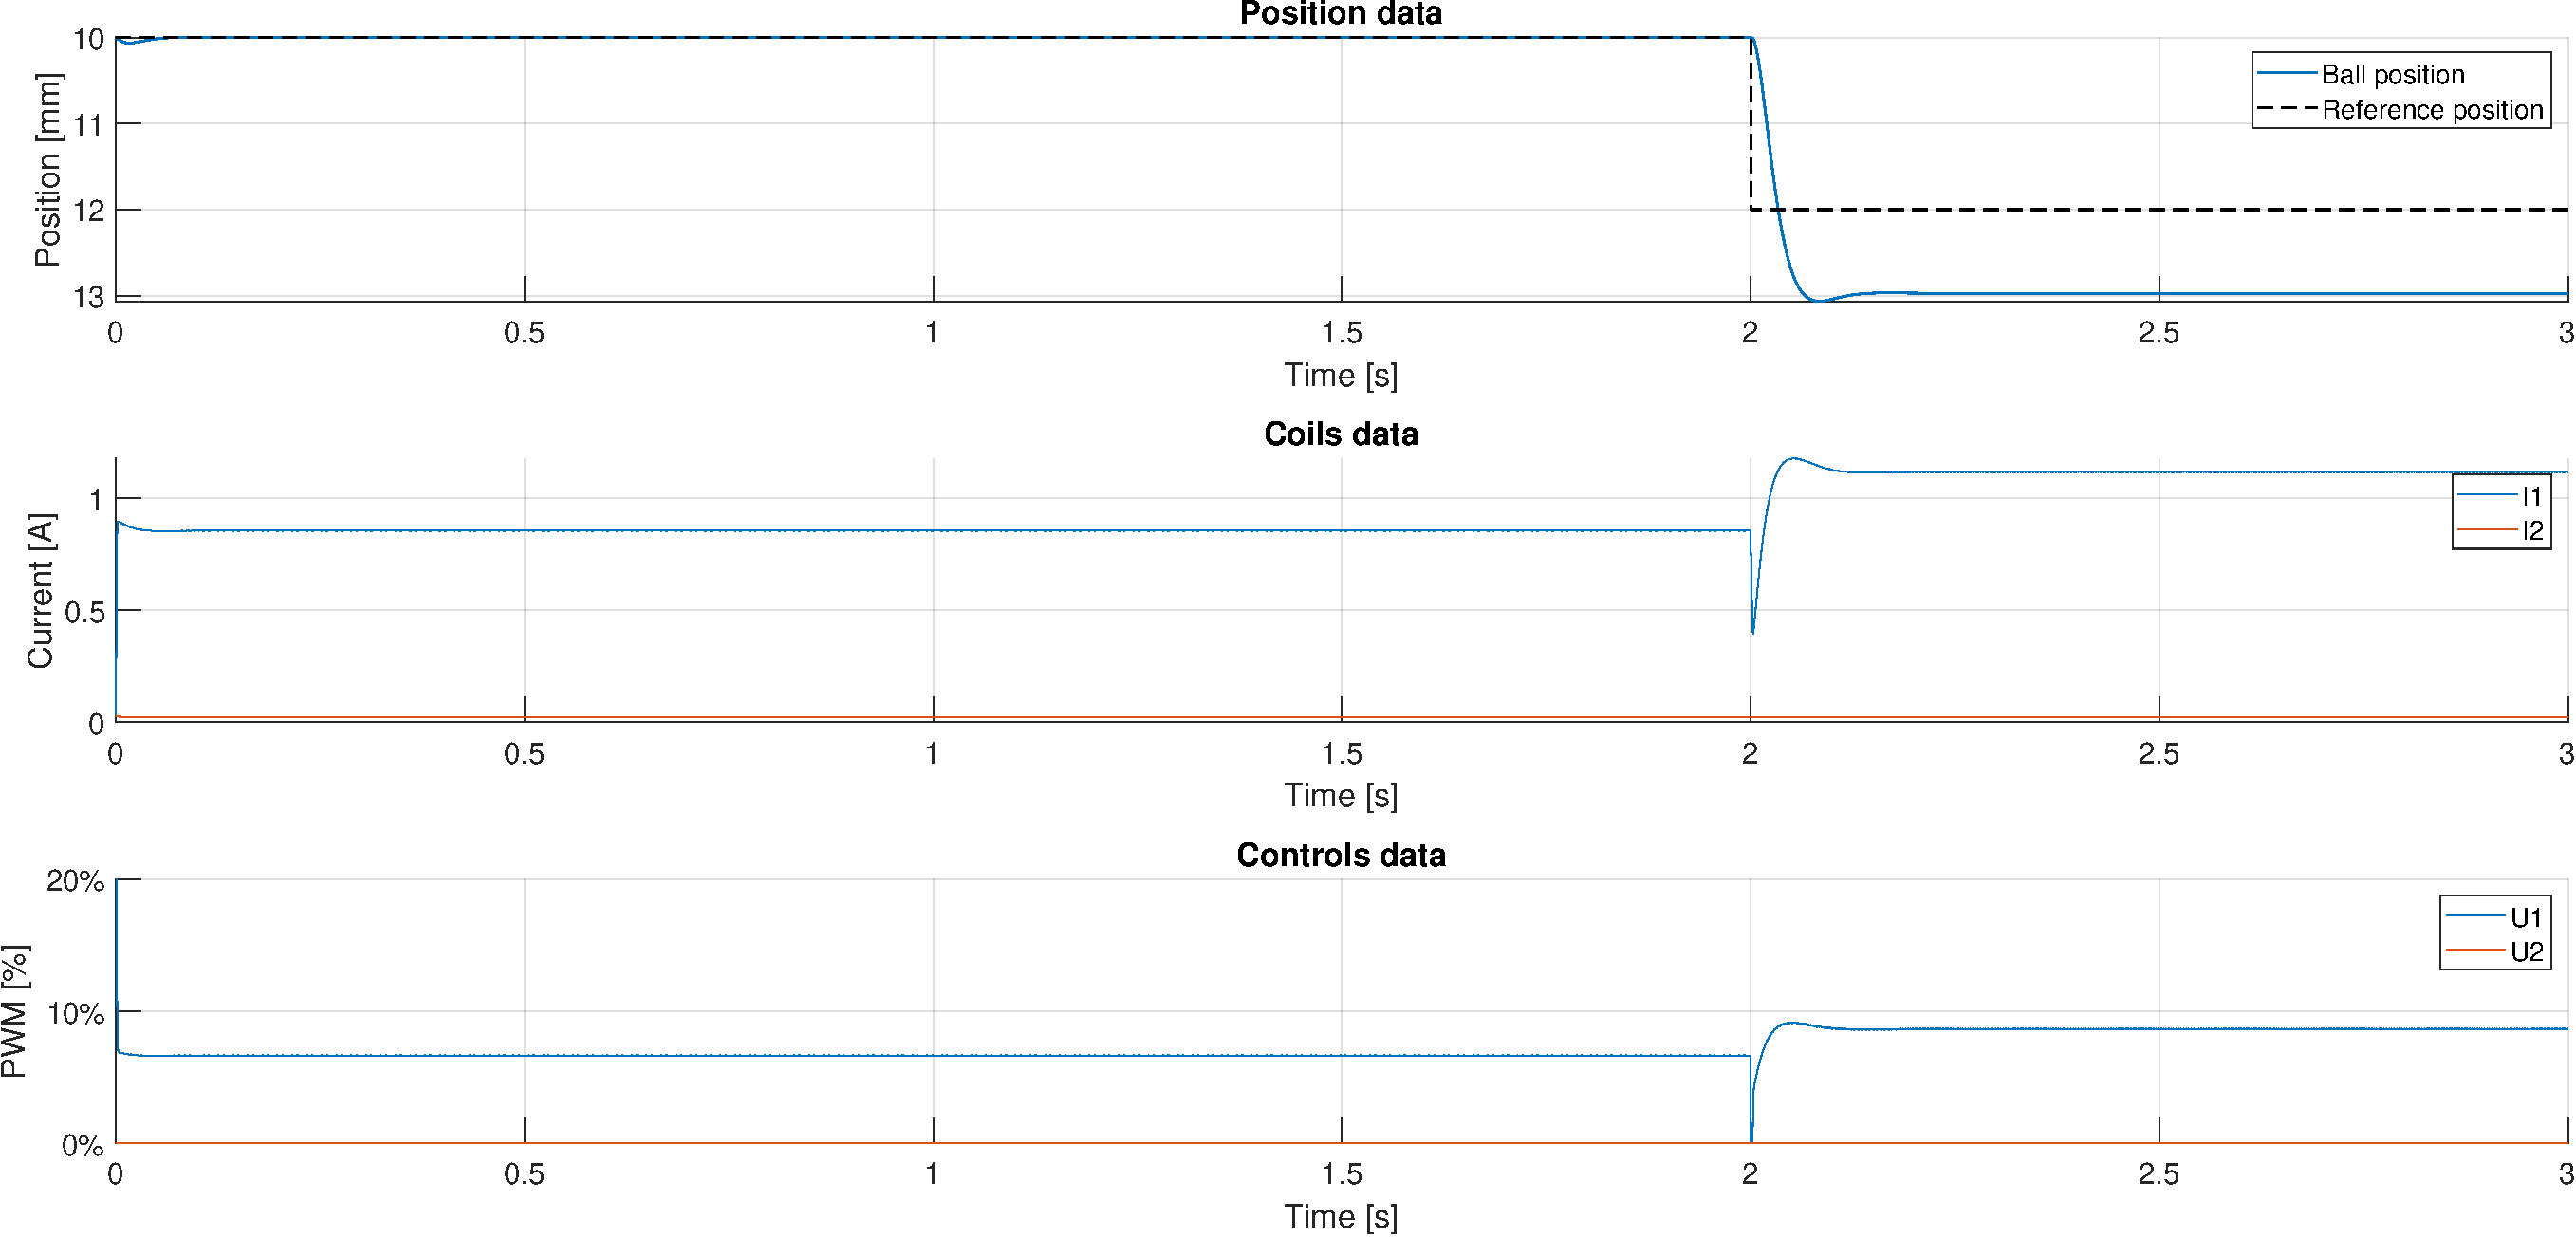
\includegraphics[width=1\textwidth]{img/MATLAB/runs/LQR_tracking.pdf}
            \caption{LQR controller}
        \end{figure}

    }

\end{frame}

